\documentclass[11pt]{article}

\usepackage[letterpaper,margin=1in]{geometry}
\usepackage[utf8]{inputenc}
\usepackage[T1]{fontenc}
\usepackage{lmodern}
\usepackage{microtype}
\usepackage{amsmath,amssymb}
\usepackage{graphicx}
\usepackage{booktabs}
\usepackage{array}
\usepackage{longtable}
\usepackage{float}
\usepackage{caption}
\usepackage{subcaption}
\usepackage{xcolor}
\usepackage{tikz}
\usetikzlibrary{arrows.meta,positioning,fit,shapes.geometric}
\usepackage{listings}
\usepackage{hyperref}
\usepackage{enumitem}
\usepackage{fancyhdr}
\usepackage{setspace}

\hypersetup{
    colorlinks=true,
    linkcolor=blue!50!black,
    citecolor=blue!50!black,
    urlcolor=blue!50!black
}

\setlist[itemize]{topsep=2pt,itemsep=2pt,parsep=0pt}
\setlist[enumerate]{topsep=2pt,itemsep=2pt,parsep=0pt}
\captionsetup{font=small,labelfont=bf}
\graphicspath{{./}{figures/}}

\setlength{\headheight}{14pt}
\pagestyle{fancy}
\fancyhf{}
\lhead{Current PBS Framework}
\rhead{VIC/Satellite Irrigation DA}
\cfoot{\thepage}

\lstdefinestyle{pythonstyle}{
    language=Python,
    basicstyle=\ttfamily\small,
    breaklines=true,
    frame=single,
    columns=fullflexible,
    showstringspaces=false,
    commentstyle=\itshape\color{gray!70!black},
    keywordstyle=\bfseries\color{blue!50!black},
    numbers=left,
    numberstyle=\tiny\color{gray!70!black},
    numbersep=6pt,
    keepspaces=true,
    upquote=true
}

\newcommand{\code}[1]{\texttt{#1}}
\newcommand{\smunits}{m$^3$ m$^{-3}$}
\newcommand{\reportfig}[4]{%
\begin{figure}[H]
\centering
\IfFileExists{#1}{%
    \includegraphics[width=#2\linewidth]{#1}%
}{%
    \fbox{\begin{minipage}[c][0.23\textheight][c]{0.90\linewidth}
    \centering
    Missing figure file for local preview:\\[3pt]
    \path{#1}\\[6pt]
    Place the file at this relative path to render the final figure.
    \end{minipage}}%
}
\caption{#3}
\label{#4}
\end{figure}
}

\title{Current Particle Batch Smoother Framework for Irrigation Estimation\\
\large VIC/Satellite Soil-Moisture Data Assimilation Technical Report}
\author{Hayden Fu and Yingying Liu}
\date{July 2026}

\begin{document}

\maketitle

\newpage

\tableofcontents

\newpage

\section{Introduction and Objective}

Irrigation is difficult to estimate, as many of the human decisions (timing, amount, method, and field-level location) are rarely measured directly. Hydrologic and land-surface models such as VIC can simulate soil moisture, evapotranspiration, runoff, and related fluxes, but the current no-irrigation model configuration does not directly encode farmer water applications. Satellite soil moisture provides an observational signal that may contain irrigation effects, but that signal is potentially noisy and often spatially aggregated.

The working hypothesis of this project is that satellite-observed soil moisture can be used to estimate possible irrigation histories. In the PBS formulation, each particle represents one possible history of precipitation and irrigation. VIC is run for each particle, simulated soil moisture is compared to satellite observations, and particles that better match the observations receive larger posterior weights. Those weights are then traced back to the particle irrigation inputs to estimate irrigation water use.

This report documents the data inputs, the current experiments run, their implementation, and their results.

\section{Study Domain}

The basin of choice is Dry Spottedtail Creek, Nebraska. The first complete sequential $\Delta SM$ test used July 1-28, 2020, divided into four weekly windows. The extended experiment then expanded the same framework to an assumed full irrigation season, May 1-September 30, 2020. Both experiments used an ensemble size of $N=100$ particles.

For the July experiment, the VIC particle ensemble was initialized from the existing \code{basin0} state on 2020-06-30. For the May-September experiment, VIC was first run for a one-year warm-up period from 2019-05-01 through 2020-04-30. This spin-up was run as a zero-irrigation open-loop VIC simulation using the same \code{basin0} forcing/parameter setup, and the final spin-up state was used as the initial state for the first PBS window on 2020-05-01. The purpose was to reduce sensitivity to arbitrary initial soil-moisture storage before the irrigation-season assimilation window.

\section{Datasets and Preprocessing}

The absolute-SM experiments use filtered observed SMAP soil moisture and an MLP trained to estimate bias between SMAP soil moisture and VIC surface moisture. In the absolute-SM likelihood, the comparison target is therefore the satellite reading minus the predicted structural bias: 

\begin{equation}
\widehat{SM}^{\,i}_{sat,t} = SM^{i}_{VIC,t} + \widehat{b}_{MLP,t},
\label{eq:mlp_bias}
\end{equation}

where $SM^{i}_{VIC,t}$ is the particle surface-layer VIC soil moisture and $\widehat{b}_{MLP,t}$ is the predicted SMAP-VIC bias.

\subsection{SMAP L3 Inputs for \texorpdfstring{$\Delta SM$}{Delta SM}}

The $\Delta SM$ experiments use SMAP L3 soil moisture from product \code{SPL3SMP\_E}. SMAP retrievals were extracted for the HUC8 domain and then paired either as weekly endpoint diagnostics or as daily within-window changes for PBS weighting. Currently, only recommended, high-quality retrievals are used in the target construction; lower-quality retrievals are treated as noisy and excluded. Using a 2020 cropland data layer (CDL), the regions of \code{cropland\_like} and \code{noncropland\_control} were separated with a CDL mask. The control region is used as a reference for evaluating whether cropland wetting is larger than nearby noncropland wetting.

Precipitation for the diagnostic comparisons comes from the existing \code{basin0} VIC forcing/output summary, specifically the daily \code{basin\_mean\_out\_prec} field. It is used to interpret wetting events but is not yet directly included in the $\Delta SM$ likelihood. This keeps the precipitation reference consistent with the VIC open-loop and particle simulations, although the SMAP cropland/control aggregates still cover the broader HUC8 domain.

\section{Current PBS Methodology}

\subsection{Workflow Overview}

Figure~\ref{fig:workflow} summarizes the current workflow. In sum, an ensemble of particles is created, 

\begin{figure}[H]
\centering
\resizebox{\textwidth}{!}{%
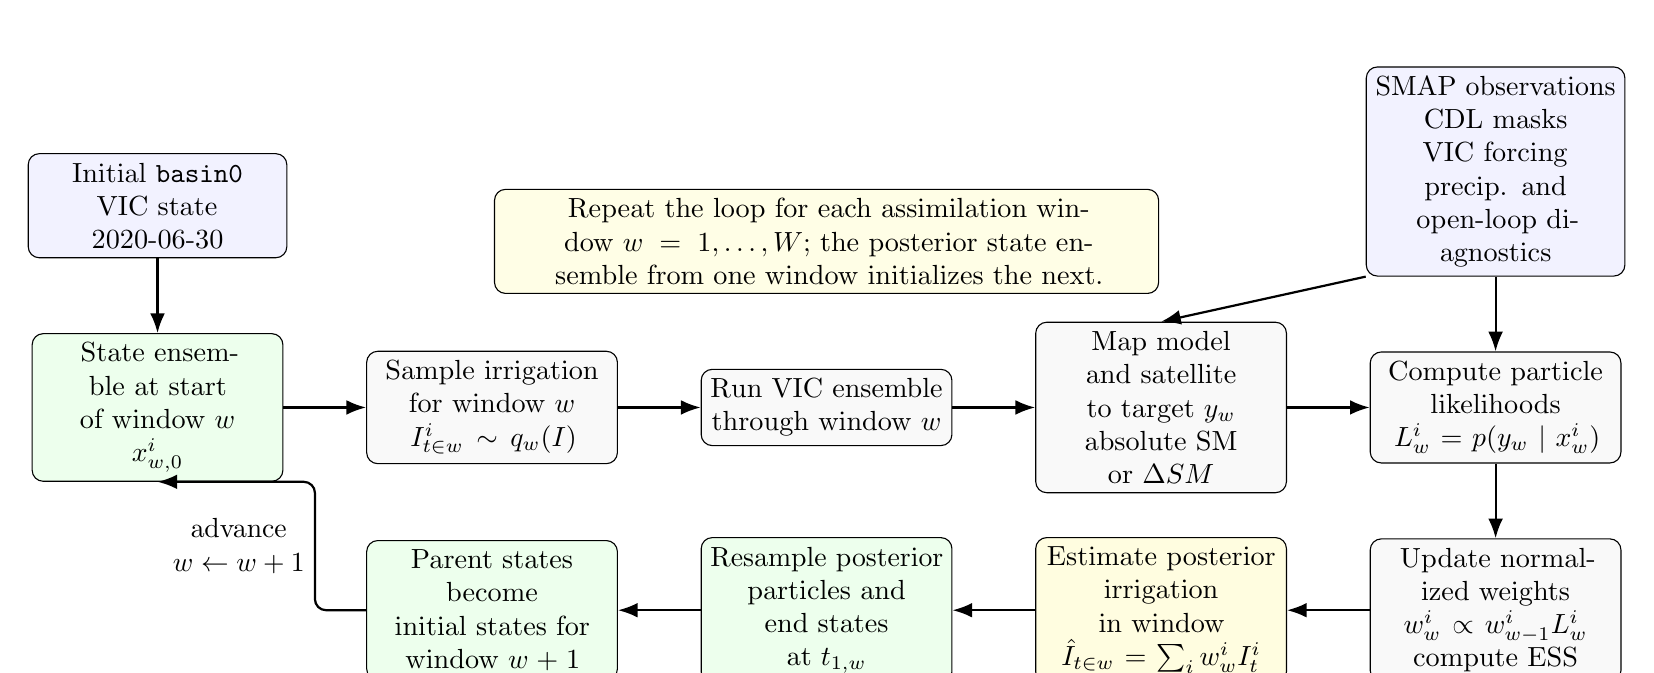
\begin{tikzpicture}[
    node distance=0.95cm and 1.05cm,
    block/.style={rectangle,draw,rounded corners,align=center,text width=2.95cm,minimum height=0.95cm,fill=gray!5},
    data/.style={rectangle,draw,rounded corners,align=center,text width=3.05cm,minimum height=0.95cm,fill=blue!5},
    state/.style={rectangle,draw,rounded corners,align=center,text width=2.95cm,minimum height=0.95cm,fill=green!7},
    result/.style={rectangle,draw,rounded corners,align=center,text width=2.95cm,minimum height=0.95cm,fill=yellow!12},
    note/.style={rectangle,draw,rounded corners,align=center,text width=8.2cm,minimum height=0.7cm,fill=yellow!10},
    arrow/.style={-{Latex[length=2.5mm]},thick},
    looparrow/.style={-{Latex[length=2.5mm]},thick,rounded corners}
]
\node[state] (state0) {State ensemble at start\\of window $w$\\$x^i_{w,0}$};
\node[block, right=of state0] (sample) {Sample irrigation\\for window $w$\\$I^i_{t\in w}\sim q_w(I)$};
\node[block, right=of sample] (vic) {Run VIC ensemble\\through window $w$};
\node[block, right=of vic] (obsop) {Map model and satellite\\to target $y_w$\\absolute SM or $\Delta SM$};
\node[block, right=of obsop] (like) {Compute particle\\likelihoods\\$L^i_w=p(y_w\mid x^i_w)$};

\node[block, below=of like] (weights) {Update normalized weights\\$w^i_w \propto w^i_{w-1}L^i_w$\\compute ESS};
\node[result, left=of weights] (post) {Estimate posterior\\irrigation in window\\$\hat{I}_{t\in w}=\sum_i w^i_w I^i_t$};
\node[state, left=of post] (resample) {Resample posterior\\particles and end states\\at $t_{1,w}$};
\node[state, left=of resample] (nextstate) {Parent states become\\initial states for\\window $w+1$};

\node[data, above=of like] (obsdata) {SMAP observations\\CDL masks\\VIC forcing precip. and\\open-loop diagnostics};
\node[data, above=of state0] (init) {Initial \code{basin0}\\VIC state\\2020-06-30};
\node[note, above=of vic] (loopnote) {Repeat the loop for each assimilation window $w=1,\ldots,W$; the posterior state ensemble from one window initializes the next.};

\draw[arrow] (init) -- (state0);
\draw[arrow] (state0) -- (sample);
\draw[arrow] (sample) -- (vic);
\draw[arrow] (vic) -- (obsop);
\draw[arrow] (obsop) -- (like);
\draw[arrow] (like) -- (weights);
\draw[arrow] (weights) -- (post);
\draw[arrow] (post) -- (resample);
\draw[arrow] (resample) -- (nextstate);
\draw[arrow] (obsdata.south west) -- (obsop.north);
\draw[arrow] (obsdata) -- (like);
\draw[looparrow] (nextstate.west) -- ++(-0.65,0) |- node[pos=0.25,left,align=center] {advance\\$w\leftarrow w+1$} (state0.south);
\end{tikzpicture}%
}
\caption{Window-by-window PBS workflow for the irrigation-estimation experiment. Each window starts from a particle state ensemble, samples candidate irrigation inputs, runs VIC over that window, maps the model and satellite observations into an absolute-SM or $\Delta SM$ target, computes likelihoods and posterior weights, estimates irrigation, and then resamples end-of-window state files to initialize the next window.}
\label{fig:workflow}
\end{figure}

\subsection{Irrigation Prior}

For each particle $i$ and day $t$, irrigation occurrence is sampled as an independent Bernoulli event:

\begin{equation}
Z^i_t \sim \mathrm{Bernoulli}(p), \qquad p = 0.25.
\label{eq:event}
\end{equation}

If an event occurs, the event amount is sampled uniformly between 5 and 30 mm/day:

\begin{equation}
I^i_t =
\begin{cases}
0, & Z^i_t = 0,\\
\mathrm{Uniform}(5,30), & Z^i_t = 1.
\end{cases}
\label{eq:irrig_prior}
\end{equation}

The total water input used to force VIC is

\begin{equation}
U^i_t = P^{obs}_t + I^i_t,
\label{eq:total_water}
\end{equation}

where $P^{obs}_t$ is observed precipitation. The added irrigation is distributed evenly across the 8 VIC model timesteps within each day and is spatially uniform across the \code{basin0} forcing grid.

For the 28-day N100 ensemble, the actual prior table contains 2,800 particle-day rows. The event fraction is 0.2329, the positive event amount range is 5.04-29.92 mm/day, and the mean number of event days per particle is 6.52.

\subsection{Likelihood and Weight Update}

For a generic observation residual $r^i_w$ for particle $i$ in window $w$, the current likelihood uses a Gaussian residual model:

\begin{equation}
\log L^i_w = -\frac{1}{2}\left(\frac{r^i_w}{\sigma}\right)^2.
\label{eq:loglik_generic}
\end{equation}

Weights are updated sequentially as

\begin{equation}
w^i_w = \frac{w^i_{w-1}L^i_w}{\sum_{r=1}^{N}w^r_{w-1}L^r_w}.
\label{eq:weight_update}
\end{equation}

The posterior irrigation estimate for each day is the weighted average of particle irrigation inputs:

\begin{equation}
\hat{I}_t = \sum_{i=1}^{N} w^i_w I^i_t, \qquad t \in w.
\label{eq:posterior_irr}
\end{equation}

Effective sample size (ESS) is used to diagnose weight degeneracy:

\begin{equation}
ESS_w = \frac{1}{\sum_{i=1}^{N}\left(w^i_w\right)^2}.
\label{eq:ess}
\end{equation}

\subsection{AdaPBS-Style Pooled Proposal Variant}

The AdaPBS-style trial uses the same likelihood and posterior-weighting equations as the basic PBS run, but changes how candidate particles are proposed. A first N100 ensemble is scored with the absolute-SM likelihood. The resulting posterior weights are then used to estimate date-specific irrigation event frequencies and positive-event amount moments, and a second N100 candidate ensemble is sampled from that adapted proposal while retaining a prior-mixture component. The final diagnostic pools the first- and second-round candidates into an N200 set and reweights them with the absolute-SM likelihood.

This is described as AdaPBS-style rather than a complete AdaPBS/AMIS implementation because the current diagnostic does not yet include exact proposal-density mixture corrections. Its purpose here is to test whether an adaptive proposal improves particle diversity, not to define the final irrigation-estimation framework.

\subsection{\texorpdfstring{$\Delta SM$}{Delta SM} Sequential Variant}

The $\Delta SM$ framework changes the observation residual rather than the posterior-irrigation calculation. Instead of comparing absolute soil-moisture levels, each particle is scored against satellite-observed soil-moisture changes:

\begin{equation}
r^i_k = \Delta SM^{sat,crop}_{k} - \Delta SM^{i}_{VIC,k}.
\label{eq:method_delta_resid}
\end{equation}

For the final HUC8 SMAP L3 run, daily within-window residuals are summed inside each weekly PBS window:

\begin{equation}
\log L^i_w = \sum_{k \in w} -\frac{1}{2}\left(\frac{r^i_k}{\sigma_{\Delta SM}}\right)^2,
\qquad \sigma_{\Delta SM}=0.075\ \mathrm{m^3\,m^{-3}}.
\label{eq:method_delta_loglik}
\end{equation}

Weights, ESS, and posterior irrigation are then computed with the same equations above. The operational difference is that after each weekly update the posterior particles are systematically resampled, their end-of-window VIC state files initialize the next window, and VIC is rerun. Thus the $\Delta SM$ experiment uses daily satellite changes for weighting, but updates and propagates the particle state ensemble at weekly boundaries.


\section{Experiment 1a: Absolute-SM Sequential PBS}

\subsection{Observation Model}

The first 4-week experiment used daily absolute satellite soil moisture for particle weighting. For retained satellite observation $j$, the residual was

\begin{equation}
r^i_j = SM^{sat}_j - \left(SM^{i}_{VIC,j} + \widehat{b}_{MLP,j}\right),
\label{eq:absolute_resid}
\end{equation}

with residual scale $\sigma=0.035$ \smunits. With multiple observations in a weekly window, the implementation summed log likelihoods across retained observations.

\subsection{Results}

\begin{table}[H]
\centering
\caption{Absolute-SM sequential PBS window results. Posterior irrigation collapsed toward nearly zero despite a nonzero prior.}
\label{tab:absolute_results}
\begin{tabular}{rrrrrrr}
\toprule
Window & Obs. & ESS & Max $w$ & RMSE & Post. irr. & Prior irr. \\
 & & & & (\smunits) & (mm) & (mm) \\
\midrule
1 & 72 & 21.00 & 0.0476 & 0.0603 & 0.0015 & 28.2698 \\
2 & 72 & 6.11 & 0.1651 & 0.0616 & 0.0529 & 25.8783 \\
3 & 56 & 2.00 & 0.5000 & 0.0558 & 0.0000 & 28.0983 \\
4 & 84 & 1.00 & 1.0000 & 0.0761 & 0.0000 & 34.2331 \\
\midrule
Total & & & & & 0.0544 & 116.4794 \\
\bottomrule
\end{tabular}
\end{table}

The experiment confirms that the particle-generation, VIC-run, observation-filtering, likelihood, and posterior-irrigation mechanics work. However, the posterior total of 0.0544 mm is not physically plausible as a July irrigation-season estimate under the current prior. The absolute-SM likelihood appears too sensitive to level mismatch between satellite observations, VIC, and the MLP mapping.

\reportfig{figures/posterior_vs_prior_daily_irrigation_4week.png}{0.92}{Absolute-SM posterior daily irrigation compared with the prior ensemble mean. The posterior nearly collapses to zero across the 4-week window, indicating that the absolute-SM likelihood strongly favored low-irrigation particles.}{fig:absolute_posterior}

\reportfig{figures/vic_raw_mlp_satellite_sm_4week.png}{0.92}{Absolute-SM assimilation inputs over the 4-week window. This diagnostic compares raw VIC surface soil moisture, MLP-adjusted satellite-equivalent VIC soil moisture, and retained satellite observations. Large level differences between these series can dominate the absolute-SM residual.}{fig:absolute_inputs}

\section{Experiment 1b: AdaPBS-Style Pooled Absolute-SM Trial}

The adaptive-proposal trial was a two-round diagnostic. Round 1 used the initial N100 proposal. Round 2 generated another N100 candidate set from the round-1 weighted event frequency and positive-event amount moments by date, while retaining a 0.20 prior-mixture component. The final likelihood was computed over the pooled 200 candidate trajectories.

This should be considered as an AdaPBS-style adaptive proposal diagnostic, not yet a full AdaPBS implementation, because exact proposal-density mixture denominators were not included.

\begin{table}[H]
\centering
\caption{AdaPBS-style pooled absolute-SM trial results. ESS improved relative to the single N100 absolute-SM run, but the posterior still favored very low irrigation.}
\label{tab:adapbs_results}
\begin{tabular}{rrrrrrrr}
\toprule
Window & Obs. & ESS & Max $w$ & Best round & RMSE & Post. irr. & Prior irr. \\
 & & & & & (\smunits) & (mm) & (mm) \\
\midrule
1 & 72 & 74.40 & 0.0135 & 1 & 0.0550 & 0.0125 & 18.5161 \\
2 & 72 & 36.24 & 0.0277 & 1 & 0.0534 & 0.0201 & 16.6203 \\
3 & 56 & 16.02 & 0.0625 & 1 & 0.0488 & 1.4132 & 18.8669 \\
4 & 84 & 9.00 & 0.1111 & 2 & 0.0665 & 0.0000 & 22.3811 \\
\midrule
Total & & & & & & 1.4458 & 76.3844 \\
\bottomrule
\end{tabular}
\end{table}

The adaptive proposal improved weight diversity but did not solve the absolute-SM collapse problem. Because round 1 already assigned high weight to low-irrigation particles, the adapted round-2 proposal also concentrated near low event probabilities.

\reportfig{figures/effective_sample_size_by_window.png}{0.82}{Effective sample size by window for the AdaPBS-style pooled run. Pooling additional adapted candidates improved ESS relative to the single N100 absolute-SM experiment, but the posterior irrigation estimate remained close to zero.}{fig:adapbs_ess}

\section{Experiment 2: HUC8 SMAP L3 \texorpdfstring{$\Delta SM$}{Delta SM} Sequential PBS}

\subsection{Experiment Design}

The final $\Delta SM$ experiment is a 4-week sequential PBS run that updates the particle state ensemble once per weekly assimilation window while using all available daily within-window SMAP L3 $\Delta SM$ targets in the likelihood. This keeps the state-update frequency at the weekly scale, where particle degeneracy is easier to manage, but still uses more than one satellite interval inside each window.

The main conceptual advantage of $\Delta SM$ is that particles are scored on changes in soil moisture rather than absolute soil-moisture level. This reduces sensitivity to static VIC-SMAP bias while preserving wetting/drying information that may reflect irrigation. The run used HUC8 \code{10180009} \code{cropland\_like} SMAP L3 targets and a working likelihood scale of $\sigma=0.075$ \smunits.

\subsection{Satellite and VIC \texorpdfstring{$\Delta SM$}{Delta SM} Targets}

SMAP L3 enhanced passive soil-moisture retrievals were extracted over HUC8 \code{10180009} and classified with the 2020 CDL crop mask. Consecutive high-quality same-cell/same-period observations were paired when both endpoints fell inside the same 7-day PBS window and the gap was 1--3 days. For SMAP cell $c$ and interval target $k$, the satellite change is

\begin{equation}
\Delta SM^{sat}_{c,k} = SMAP_{c}(t_{1,k}) - SMAP_{c}(t_{0,k}).
\label{eq:sat_delta_cell}
\end{equation}

The cell-level changes were then aggregated over the cropland-like mask using HUC8 overlap-area weights:

\begin{equation}
\Delta SM^{sat,crop}_{k} =
\frac{\sum_{c \in crop} A_c \Delta SM^{sat}_{c,k}}{\sum_{c \in crop} A_c}.
\label{eq:sat_delta_crop}
\end{equation}

This produced 5, 6, 7, and 5 aggregate daily target rows across windows 1--4.

\begin{lstlisting}[style=pythonstyle,caption={Simplified daily within-window $\Delta SM$ target construction.},label={lst:delta_target}]
for window in weekly_windows:
    for cell in huc8_smap_cells:
        obs = good_smap_obs(cell, start=window.start, end=window.end)
        for start_obs, end_obs in consecutive_same_period_pairs(obs):
            if 1 <= (end_obs.date - start_obs.date).days <= 3:
                delta_sm_cell = end_obs.soil_moisture - start_obs.soil_moisture
                save_interval_delta(cell, start_obs, end_obs, delta_sm_cell)

sat_crop_delta = area_weighted_mean(delta_sm_cell, mask_class="cropland_like")
\end{lstlisting}

\subsection{Particle \texorpdfstring{$\Delta SM$}{Delta SM}, Likelihood, and State Update}

For the VIC open-loop reference,

\begin{equation}
\Delta SM^{VIC,OL}_w = SM^{VIC,OL}(t_{1,w}) - SM^{VIC,OL}(t_{0,w}).
\label{eq:vic_open_loop_delta}
\end{equation}

For each particle and interval,

\begin{equation}
\Delta SM^{i}_{k} = SM^{i}_{VIC}(t_{1,k}) - SM^{i}_{VIC}(t_{0,k}).
\label{eq:particle_delta}
\end{equation}

The daily \code{cropland\_only} residual is

\begin{equation}
r^i_k = \Delta SM^{sat,crop}_{k} - \Delta SM^{i}_{k}.
\label{eq:delta_resid}
\end{equation}

For window $w$, residual likelihoods were summed across all available daily interval targets in that window:

\begin{equation}
\log L^i_w = \sum_{k \in w} -\frac{1}{2}\left(\frac{r^i_k}{0.075}\right)^2.
\label{eq:delta_loglik}
\end{equation}

The 0.075 \smunits{} scale is a working assumption, not an independently calibrated observation-error model.

\begin{lstlisting}[style=pythonstyle,caption={Simplified implementation of the daily $\Delta SM$ likelihood and sequential update.},label={lst:delta_likelihood}]
sigma = 0.075
log_likelihood = 0.0
for target in daily_targets_in_window:
    residual = target.sat_crop_delta_sm - particle_delta_sm[target.interval]
    log_likelihood += -0.5 * (residual / sigma) ** 2

# Stabilize exponentiation before multiplying by prior weights.
likelihood = np.exp(log_likelihood - np.max(log_likelihood))
weights = prior_weights * likelihood
weights = weights / weights.sum()
ess = 1.0 / np.sum(weights ** 2)

parent_particles = systematic_resample(weights)
next_window_initial_states = end_states[parent_particles]
\end{lstlisting}

Operationally, the workflow runs one 7-day VIC ensemble at a time. After the likelihood update, posterior weights are used for systematic resampling, and the selected end-of-window state files initialize the next weekly ensemble. 

\subsection{Results}

\begin{table}[H]
\centering
\caption{Completed Week 7 daily $\Delta SM$ sequential PBS results.}
\label{tab:delta_primary_results}
\resizebox{\textwidth}{!}{%
\begin{tabular}{rrrrrrrrr}
\toprule
Window & Daily obs & ESS & Max $w$ & Best particle & Post. irr. & Prior irr. & Unique parents & Max offspring \\
 & & & & & (mm) & (mm) & & \\
\midrule
1 & 5 & 40.32 & 0.030 & 0 & 12.3798 & 28.8987 & 47 & 3 \\
2 & 6 & 27.85 & 0.047 & 79 & 5.8403 & 28.9926 & 38 & 5 \\
3 & 7 & 39.58 & 0.036 & 84 & 13.6089 & 29.3866 & 44 & 4 \\
4 & 5 & 22.80 & 0.063 & 48 & 9.3124 & 31.7017 & -- & -- \\
\midrule
Total & & & & & 41.1413 & 118.9795 & & \\
\bottomrule
\end{tabular}%
}
\end{table}

The posterior total is 41.14 mm, compared with a prior mean of 118.98 mm. The result is clearly nonzero, but much lower than the irrigation prior. The minimum ESS remained 22.80, so the daily $\Delta SM$ likelihood did not collapse onto a single particle under the selected $\sigma=0.075$ scale. Parent-particle diversity also remained moderate across the resampling steps.

\reportfig{figures/posterior_vs_prior_daily_irrigation_resample_rerun.png}{0.92}{Posterior daily irrigation from the completed daily $\Delta SM$ sequential PBS experiment. The daily timing comes from weighted stochastic particle proposals within each weekly window.}{fig:resample_rerun_daily_irr}

\reportfig{figures/effective_sample_size_by_window_resample_rerun.png}{0.78}{Effective sample size by window for the completed daily $\Delta SM$ sequential PBS experiment.}{fig:resample_rerun_ess}

\reportfig{figures/resampling_parent_diversity.png}{0.78}{Number of unique parent particles selected during systematic resampling for the next weekly window.}{fig:resample_parent_diversity}

\section{Experiment 2b: Full-Season HUC8 SMAP L3 \texorpdfstring{$\Delta SM$}{Delta SM} Sequential PBS}

\subsection{Extended-Season Design}

The next experiment extended the Experiment 2 workflow from a 4-week July diagnostic to an assumed full irrigation season, May 1-September 30, 2020. The goal was not to change the PBS framework, but to test whether the same daily $\Delta SM$ sequential method could run over a realistic season length and produce interpretable irrigation timing. The full-season run used the same HUC8 \code{10180009} SMAP L3 \code{cropland\_like} target, the same weekly state-resampling/rerun structure, and the same working likelihood scale of $\sigma_{\Delta SM}=0.075$ \smunits.

Before the PBS period, VIC was run for one year from 2019-05-01 to 2020-04-30 to generate an initial hydrologic state. This spin-up was a zero-irrigation open-loop VIC run using the existing \code{basin0} setup. Its end-of-run state initialized the first seasonal PBS window beginning on 2020-05-01. The spin-up is important because a May 1 start date is earlier than the July proof-of-concept, and the model soil-moisture state entering the irrigation season should reflect a physically evolved antecedent condition rather than an arbitrary cold start.

The May-September PBS period was divided into 22 weekly windows. As in Experiment 2, each window sampled a fresh daily irrigation proposal for 100 particles, ran VIC through that window, scored particles against daily within-window SMAP L3 $\Delta SM$ targets, resampled posterior states, and passed the selected end states to the next window.

\subsection{Results}

\begin{table}[H]
\centering
\caption{Full-season May-September 2020 daily $\Delta SM$ sequential PBS results.}
\label{tab:season_delta_results}
\resizebox{\textwidth}{!}{%
\begin{tabular}{rllrrrrr}
\toprule
Window & Start & End & Daily obs & ESS & Max $w$ & Post. irr. & Prior irr. \\
 & & & & & & (mm) & (mm) \\
\midrule
1 & 2020-05-01 & 2020-05-07 & 10 & 11.82 & 0.180 & 41.6301 & 37.0662 \\
2 & 2020-05-08 & 2020-05-14 & 10 & 31.84 & 0.056 & 15.6553 & 30.7054 \\
3 & 2020-05-15 & 2020-05-21 & 8 & 31.83 & 0.085 & 19.0077 & 32.2485 \\
4 & 2020-05-22 & 2020-05-28 & 9 & 34.33 & 0.046 & 14.3405 & 29.3432 \\
5 & 2020-05-29 & 2020-06-04 & 8 & 19.66 & 0.093 & 8.0269 & 31.6068 \\
6 & 2020-06-05 & 2020-06-11 & 9 & 4.84 & 0.396 & 37.7000 & 31.5989 \\
7 & 2020-06-12 & 2020-06-18 & 9 & 22.49 & 0.057 & 4.6586 & 29.1275 \\
8 & 2020-06-19 & 2020-06-25 & 6 & 43.59 & 0.050 & 21.8138 & 28.8238 \\
9 & 2020-06-26 & 2020-07-02 & 10 & 18.54 & 0.088 & 14.9272 & 34.1503 \\
10 & 2020-07-03 & 2020-07-09 & 10 & 18.63 & 0.082 & 4.3909 & 27.5025 \\
11 & 2020-07-10 & 2020-07-16 & 6 & 25.20 & 0.051 & 5.8447 & 27.3689 \\
12 & 2020-07-17 & 2020-07-23 & 12 & 19.66 & 0.066 & 14.0895 & 27.0350 \\
13 & 2020-07-24 & 2020-07-30 & 9 & 24.76 & 0.054 & 5.7480 & 29.0778 \\
14 & 2020-07-31 & 2020-08-06 & 7 & 29.95 & 0.041 & 12.1869 & 29.6064 \\
15 & 2020-08-07 & 2020-08-13 & 10 & 17.66 & 0.072 & 6.0977 & 33.7825 \\
16 & 2020-08-14 & 2020-08-20 & 8 & 19.59 & 0.073 & 8.5742 & 33.9076 \\
17 & 2020-08-21 & 2020-08-27 & 10 & 23.21 & 0.051 & 3.1406 & 30.8018 \\
18 & 2020-08-28 & 2020-09-03 & 10 & 15.08 & 0.074 & 1.0158 & 29.1995 \\
19 & 2020-09-04 & 2020-09-10 & 8 & 25.91 & 0.070 & 11.1421 & 32.2942 \\
20 & 2020-09-11 & 2020-09-17 & 11 & 23.55 & 0.070 & 5.3567 & 27.4037 \\
21 & 2020-09-18 & 2020-09-24 & 8 & 21.38 & 0.055 & 2.5425 & 28.4646 \\
22 & 2020-09-25 & 2020-09-30 & 7 & 25.82 & 0.043 & 2.4383 & 23.6451 \\
\midrule
Total & & & & & & 260.3281 & 664.7603 \\
\bottomrule
\end{tabular}%
}
\end{table}

The full-season posterior total was 260.33 mm, compared with a prior mean of 664.76 mm. As in the July experiment, the $\Delta SM$ likelihood substantially reduced the irrigation implied by the stochastic prior while retaining a clearly nonzero posterior estimate. The seasonal posterior is concentrated more heavily in May and June, with much smaller daily irrigation estimates through late August and September. This timing is visible in the posterior irrigation time series and is broadly consistent with the particle weights favoring stronger early-season wetting histories.

The main caution is weight degeneracy in window 6, covering 2020-06-05 to 2020-06-11. That window had the minimum seasonal ESS of 4.84 and the largest single-particle weight of 0.396. The corresponding resampling step selected only 25 unique parents for the next window, with one parent contributing 40 offspring. This does not invalidate the run, but it identifies window 6 as the first target for closer diagnosis. It may reflect a particularly sharp satellite $\Delta SM$ target, a rainfall/soil-moisture timing mismatch, or too small an effective likelihood scale for that week.

\reportfig{figures/season_abolafia_rosenzweig_style_delta_sm_pbs_diagnostic.png}{0.98}{Full-season $\Delta SM$ PBS diagnostic for May-September 2020. Particle soil-moisture trajectories are colored from light to dark purple by relative posterior weight within each weekly window. Red points show area-weighted cropland-like SMAP L3 soil moisture, the black line shows the weighted ensemble mean, the dashed black line shows open-loop VIC, and blue bars show VIC forcing precipitation on the right-hand axis.}{fig:season_delta_pbs_diagnostic}

\reportfig{figures/season_posterior_vs_prior_daily_irrigation_resample_rerun.png}{0.92}{Full-season posterior daily irrigation compared with the prior ensemble mean. The posterior total is 260.33 mm versus a prior total of 664.76 mm, with larger inferred irrigation in May-June and smaller estimates later in the season.}{fig:season_posterior_irrigation}

\reportfig{figures/season_effective_sample_size_by_window_resample_rerun.png}{0.78}{Effective sample size by window for the full-season sequential $\Delta SM$ PBS run. Window 6 is the clearest degeneracy case, with ESS = 4.84.}{fig:season_ess}

\reportfig{figures/season_max_particle_weight_by_window_resample_rerun.png}{0.78}{Maximum particle weight by window for the full-season sequential $\Delta SM$ PBS run. The largest maximum weight was 0.396 in window 6.}{fig:season_max_weight}

\reportfig{figures/season_resampling_parent_diversity.png}{0.78}{Parent-particle diversity during full-season sequential resampling. The window 6 update is again the main low-diversity case, with one parent producing many offspring for the next window.}{fig:season_parent_diversity}

\section{Conclusion}

The current PBS framework is now operational enough to compare different observation formulations rather than only debug the workflow. The absolute soil-moisture experiments confirmed that the particle generation, VIC runs, likelihood calculation, and posterior irrigation recovery are functioning, but they also showed that direct absolute-SM weighting is too sensitive to level mismatch between VIC, SMAP, and the bias-correction model. Even with the AdaPBS-style pooled proposal, the posterior still favored very low irrigation, suggesting that the main issue is the observation target rather than particle mechanics alone.

The $\Delta \mathrm{SM}$ experiments are more promising. The 4-week July sequential run produced a nonzero posterior irrigation estimate of 41.14 mm from a 118.98 mm prior mean while maintaining relatively healthy particle weights. The extended May-September run then showed that the same framework can run across a full assumed irrigation season after a one-year VIC spin-up. That seasonal experiment produced a posterior total of 260.33 mm from a 664.76 mm prior mean, with the largest inferred irrigation concentrated in May and June. The seasonal run also identified one important diagnostic issue: window 6 had low ESS and a dominant particle, so that week should be examined before treating the seasonal estimate as stable.

These results should still be treated as a work in progress rather than a validated irrigation estimate. The framework still uses a simple stochastic irrigation prior, an assumed $\Delta \mathrm{SM}$ likelihood scale, and a spatial setup where the HUC8 satellite cropland/control comparison is not identical to the \code{basin0} VIC model domain. The next stage should focus on validation against independent irrigation or water-use data for the region, closer inspection of the low-ESS seasonal window, and improved physical filtering or calibration of the $\Delta \mathrm{SM}$ likelihood so that rainfall-driven, noisy, or implausible satellite changes do not receive undue weight. The main conclusion at this stage is that the $\Delta \mathrm{SM}$ PBS framework is a more promising direction than absolute-SM weighting, and the seasonal experiment is the strongest demonstration so far that it can be scaled beyond a short proof-of-concept window.

\end{document}
